


\chapter{Fundamentação Teórica}

\section{Processamento Digital de Imagens}

Processamento digital de imagens segundo \citeonline{jain1989fundamentals}, consiste na manipulação de imagens em formato digital utilizando algoritmos para extrair informações, melhorar a qualidade ou transformar dados visuais. Esta área engloba diversas técnicas que permitem o tratamento de imagens capturadas por dispositivos digitais, como câmeras e scanners, visando a otimização de aspectos como contraste, nitidez e remoção de ruído \cite{gonzalez2010processamento}. Além de aprimorar a percepção visual, essas técnicas são essenciais para a análise automática de imagens, facilitando a identificação e classificação de objetos, a medição de propriedades geométricas e a extração de padrões \cite{russ2006image}.

No processamento digital de imagens, os processos geralmente são abordados em três níveis distintos, cada um com um papel específico na análise e interpretação das imagens. O nível baixo trata de manipulações mais primitivas, realizando operações fundamentais como filtragem, aprimoramento de contraste e remoção de ruído. O nível médio foca na segmentação e extração de características, onde a imagem é dividida em regiões de interesse e características relevantes são identificadas e descritas. Finalmente, o nível alto envolve a interpretação e reconhecimento dos dados processados, onde algoritmos são aplicados para classificar objetos, reconhecer padrões e realizar decisões baseadas em informações extraídas dos níveis anteriores. Cada um desses níveis do processamento de imagens contribui de maneira distinta para a análise visual, formando uma cadeia de processamento que vai desde a manipulação básica até a interpretação complexa \cite{gonzalez2010processamento}. 

Ainda segundo \citeonline{gonzalez2010processamento} o processamento digital de imagens envolve uma série de passos que vão desde a aquisição até interpretação das imagens. Como pode ser visto na Figura \ref{etapasProcessamentoImagens}, essas etapas incluem:


\begin{enumerate}
    \item \textbf{Aquisição de Imagem}: Este estágio trata da obtenção de imagens, que podem ser capturadas por dispositivos digitais ou provenientes de arquivos digitais já existentes. Neste processo, podem ser realizados ajustes iniciais, como modificar o tamanho da imagem.
    
    \item \textbf{Filtragem e realce de imagens}: Nesta fase, a imagem é manipulada para adequá-la a uma aplicação específica. Em alguns casos, como em imagens médicas, a melhoria pode não ser a abordagem mais apropriada.

    \item \textbf{Restauração de imagens}: Este passo busca aprimorar a qualidade visual das imagens através de métodos baseados em modelos matemáticos ou probabilísticos para compensar a degradação da imagem.

    \item \textbf{Processamento de Imagens em Cores}: Com o aumento do uso de imagens digitais na web, o processamento de imagens coloridas tornou-se fundamental. Trabalhar com cores facilita a extração de características relevantes de uma imagem.

    \item \textbf{Processamento em Multiresolução}: Este método envolve a representação de uma imagem em diferentes níveis de resolução, permitindo uma análise detalhada em várias escalas.

    \item \textbf{Compressão de Imagem}: Nesta fase, são aplicadas técnicas para armazenar imagens de maneira mais eficiente ou reduzir a largura de banda necessária para sua transmissão.

    \item \textbf{Processamento Morfológico}: O processamento morfológico foca na extração e análise dos componentes da imagem para descrever suas formas.

    \item \textbf{Segmentação}: A segmentação é um dos aspectos mais desafiadores no processamento digital de imagens. Ela consiste em dividir a imagem em partes ou objetos distintos.

    \item \textbf{Representação e Descrição de Características}: Este processo, também conhecido como seleção de atributos, visa extrair características que forneçam informações quantitativas ou qualitativas para distinguir entre diferentes tipos de objetos.

    \item \textbf{Identificação de Objetos}: O reconhecimento de objetos é o processo de atribuir rótulos a elementos presentes em uma imagem, como classificar um objeto como um "carro".

    \item \textbf{Base de conhecimento}: Envolve o entendimento do domínio do problema, incluindo informações detalhadas sobre áreas específicas na imagem onde se espera encontrar dados relevantes.

    
\end{enumerate}

\begin{figure}
    \centering   
    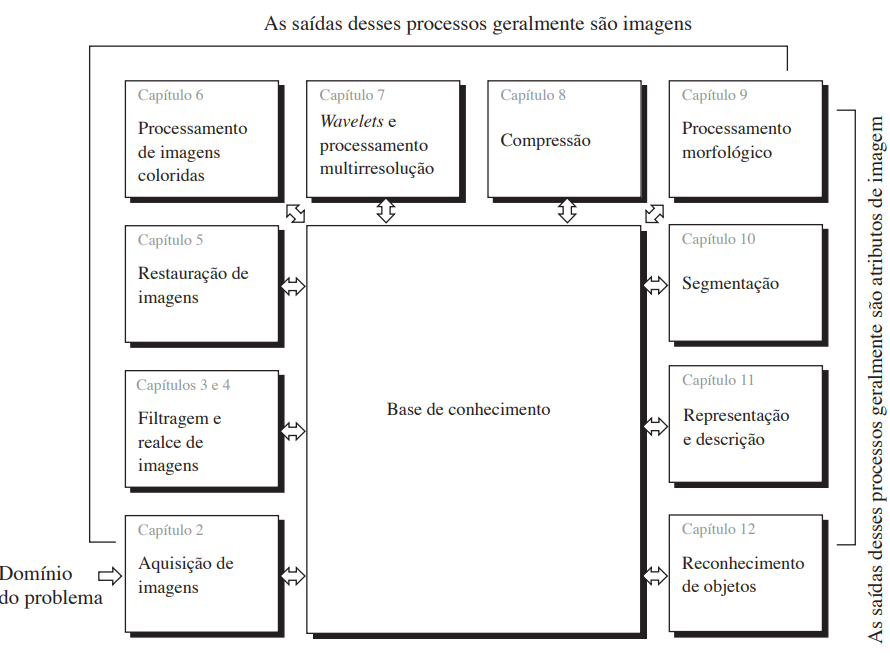
\includegraphics[width=\textwidth]{fig/PassosProcessamentoDigitalDeImagens.png}
    \caption{Etapas do processamento digital de imagens que vai desde a aquisição de imagens até a identificação e descrição de objetos presente nelas.}
    \label{etapasProcessamentoImagens}
\end{figure}

O processamento digital de imagens é amplamente aplicado em áreas como a medicina, para a análise de imagens de diagnóstico, na indústria, para o controle de qualidade de produtos, na segurança, para reconhecimento facial e monitoramento e entre outros \cite{gonzalez2010processamento}. %https://archive.org/details/imageprocessingh03edruss




\subsection{Transformação de Intensidade}


As transformações de intensidade são técnicas no processamento digital de imagens focadas na manipulação direta dos valores de intensidade dos pixels. Elas operam individualmente em cada pixel, possibilitando ajustes de contraste, brilho e outros atributos de uma imagem. O objetivo principal dessas transformações é modificar a aparência visual da imagem para realçar características específicas ou preparar a imagem para análises posteriores \cite{gonzalez2010processamento}.

% No processamento digital, cada pixel de uma imagem é representado por um valor de intensidade, que pode ser ajustado através de uma transformação matemática. A relação entre os valores de intensidade antes e depois da transformação é descrita pela função $𝑠=𝑇(𝑟)$, onde $𝑟$ é o valor de intensidade original, $𝑠$ é o valor de intensidade transformado, e $𝑇$ é a função de transformação. Esses valores são manipulados usando tabelas indexadas, especialmente em ambientes de 8 bits, onde a tabela contém 256 entradas para mapear os valores de $𝑟$ em $𝑠$.

% gonzales pag 55 e 69 operações basicas da transformação de intensidade
As principais funções de transformação de intensidade incluem:

\textbf{Transformações Lineares:} Essas funções incluem transformações como o negativo e a identidade. A transformação de negativo inverte os valores de intensidade, enquanto a identidade mantém os valores de intensidade inalterados.

\textbf{Transformações Logarítmicas:} Essas funções utilizam operações logarítmicas para alterar a distribuição de intensidade. Transformações como o logaritmo e o logaritmo inverso são utilizadas para melhorar detalhes em áreas escuras da imagem ou para estender o alcance dinâmico.

\textbf{Transformações de Potência:} Utilizam funções de potência e raiz para ajustar o contraste e a gama da imagem. Transformações de n-ésima potência e n-ésima raiz são exemplos de como essas funções podem ajustar as características da imagem.

Assim, ao aplicar transformações de intensidade e técnicas de filtragem, é possível ajustar e melhorar imagens de maneira significativa, seja para visualização aprimorada ou para análises mais precisas.
% EXEMPLO optional
Considere a transformação de intensidade ilustrada na Figura \ref{exemploTransformacaoIntensidade}.a. Como mostra \citeonline{gonzalez2010processamento}, quando aplicamos essa transformação a cada pixel da imagem original $f$, geramos uma nova imagem $g$ com maior contraste. Nesta transformação, os valores de intensidade abaixo de um ponto $k$ são escurecidos, enquanto os valores acima de $k$ são clareados. Isso resulta em uma imagem com contraste ampliado, onde áreas escuras são mais densas e áreas claras são mais evidentes.

Na Figura \ref{exemploTransformacaoIntensidade}.b, a transformação $T(r)$ resulta em uma imagem binária, onde os pixels são convertidos em apenas dois níveis de intensidade, dependendo de um limiar específico. Essa técnica, conhecida como limiarização, simplifica a imagem original em uma forma mais clara e destacada, com apenas duas cores, tipicamente preto e branco.

Essas transformações são exemplos de como ajustes nos valores de intensidade podem alterar significativamente a aparência e a utilidade da imagem, dependendo do objetivo do processamento.

\begin{figure}
    \centering   
    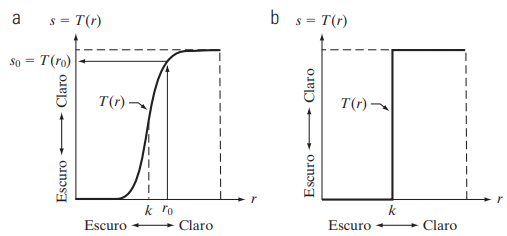
\includegraphics[width=\textwidth]{fig/ExemploTranformacaoIntensidade.png}
    \caption{Funções para ajuste da intensidade em imagens. (a) Método de ampliação de contraste, que aumenta a diferença entre os níveis de intensidade, destacando áreas mais escuras e mais claras. (b) Método de binarização, que converte a imagem em dois níveis distintos de intensidade, geralmente preto e branco, com base em um limiar definido.}
    \label{exemploTransformacaoIntensidade}
\end{figure}

\section{Deep Learning}

\section{Informação de profundidade}
Sensores de profundidade estão cada vez mais embarcados em equipamentos amplamente difundidos como dispositivos de realidade aumentada (Occulus, Kinnect) e até mesmo em smartphones \cite{du2020depthlab}, principalmente as câmeras ToF, pois são capazes de desempenhar de maneira satisfatória mesmo com baixa potência \cite{branscombe2018microsoft}. De acordo com \cite{xie2021ultradepth}, a adoção de sensores de profundidade em smartphones tende a aumentar nos próximos anos, com diversas aplicações como tradução de linguagem de sinais \cite{park2021enabling} e sistemas de navegação mobile para pessoas com deficiência visual \cite{see2022smartphone}.

%sinal 57, gestos 86, e aumentada 97

Ainda segundo \cite{castellano2023performance}, cada uma das técnicas de aquisição de imagens de profundidade possui lados negativos que podem impactar os dados. Por exemplo, as câmeras ToF podem sofrer com invalidação de pixels próximos a cantos ou bordas de objetos devido à interferências entre os raios IR em superfícies descontínuas ou reflexivas \cite{hansard2012time}. Outros tipos de câmeras RGB-D mais comuns como o Microsoft Kinect ou Intel RealSense podem produzir valores inválidos em superfícies muito brilhantes ou reflexivas como espelhos, superfícies metálicas ou muito escuras \cite{zollhofer2019commodity}. Em ambientes internos, tais imagens podem conter até 50\% de dados faltantes. \cite{zhang2022indepth} \cite{zhang2018deep}. Pontos cuja medição é desconhecida são representados por pixels totalmente pretos ou totalmente brancos \cite{dourado2020multi}.
\section{Modelos de estimação de profundidade}
